\chapter{Halbleiter}

\underline{Charakteristika}:

\begin{itemize}
\item Metallischen Glanz aber kein Metall
\item Negativer Temperatur Koeffizient \(\rho\uparrow \quad T\downarrow\)
\item Photoleitfähigkeit
\item Eigenschaften können von Verunreinigungen empfindlich abhängen
\end{itemize}

 Materialien:
4.hauptgruppe: Si,Se, Ga,Teller, P, B,
Verbindungen III-V: GaAs, InSb
II-VI: ZnS,CdS
IV-IV: SiC


\underline{Elektrischer Widerstand}

Metall \(\rho = 10^{-7} \text{ bis } 10^{-8}\Omega m\)
isolator \(\rho > 10^{12}\Omega m \)
Halbleiter \(\rho = 10^{-4} \text{ bis } 10^{7}\Omega m \)
\(\exists\) Bandlücke, kleiner als bei Isolatoren
bei T=0 Halbleiter sind Isolatoren
T>0 Wahrscheinlichkeit für eine Termische Anregung
\(E_g>0,1 ... 2eV\)
\(E\propto e^{-\frac{E_g}{2kT}}\)

\underline{Intrinsische Halbleiter}: Eigenschaften werden durch Thermische anregung bestimmt
\underline{Extrinsische Halbleiter}: Eigenschaften werden durch Dotierung von Frembatomen bestimmt


\begin{enumerate}
\item[1)] Intrinsische HL

  \begin{enumerate}
  \item[a)] Bandlücke und optische Abstände Indirekter Übergang
 Impuls wird durch Phonon gewährleistet; 
    \underline{ Kristallimpulserhaltung}
Übergang hängt von  Phononenspektrum ab und daher von der Temperatur abhängig. Photon: große Energie, kleiner Impuls; Phonon: kleine Energie, großer Impuls

\underline{Direkter Übergang}

schwache Temperaturabhängigkeit (vgl \(1500nm\approx 0,8eV\)
  \item[b)] Effektive Massen von Elektronen und Löchern

 Bandkrümmung in der Nähe des Übergangs,; Parabolische Näherung:
\[E_n= E_L + \frac{\hbar^2 k^2}{2m^*}\]

mit n=Elektronen und p=Löcher. Elektronen im Leitungsband im 

\begin{tabular}{ccc}
&Transversal&Longitudinal\\
  Si & \(\frac{m^*_t}{m_e}=0,19\)& \(\frac{m^*_l}{m_e}=0,19\)\\
Ge&  \(\frac{m^*_t}{m_e}=0,082\)& \(\frac{m^*_l}{m_e}=1,57\)
\end{tabular}

Löcher im Valenzband
\begin{tabular}{ccc}
&Transversal&Longitudinal\\
  Si & \(0,16mc\)& \(0,49mc\)\\
& leicht Loch& schweres Loch
\end{tabular}

\(GaAs\)
\begin{tabular}{ccc}
&Transversal&Longitudinal\\
  Löcher & \(\frac{m^*_t}{m_e}=0,12\)& \(\frac{m^*_l}{m_e}=0,61\)\\
&leicht&schwer\\
& leicht Loch& schweres Loch
\end{tabular}
 
  \item[c)] Metall-Halbleiter Übergang

Austrittsarbeit \(\phi\) zum Vakuum. Die Austrittsarbeit bestimmti die el. Eigenschaft.

n-Dotiert: \(\phi_{HL}>\phi_{ME}\) ohmscher Kontakt
\(\phi_{HL}<\phi_{ME}\) blokierender Kontakt (Schottky-Kontakt). An der Grenzfläche ensteht eine Hochohmige Verarmungszohne. Elektronen fließen ins Metall

p-Dotiert: genau andersherum



  \end{enumerate}


\item[2)] Dotierte HL

  \begin{enumerate}
  \item[a)] Spezifischer Widerstandhängtstart von der Konzentration der Verunreinigung ab.
  \item[b)] Donatoren: liefern zusätzliche Elektronen ins Leitungsband: P, As, Sb; haben eine höhere Valenz
Akzeptoren: liefern zustzliche Löcher in Valenzband. niedrigere Valenz als das Wirtsmaterial: B,Al,Ga,In

Modell: Donator verhält sich wie ein positiv geladenes Ion mit zusätzlichen Elektron. Bohr-Radius somit größer als beim H-Atom; Bindungsenergie \(\approx 10meV\)
  \end{enumerate}

\item[3)] Inhomogene HL

  \begin{enumerate}
  \item[a)] p-n Übergang


    \begin{itemize}
    \item angleichung des chem. Potentials (\(E_F\))
    \item Verarmung freier Ladungsträger im Bereich des Übergangs durch rekombination mit Ladungsträgern von anderen Typ.
    \item geladenen Störstellen bleiben zurück, es entwickelt sich eine Raumladungszone
    \end{itemize}

  \item[b)] Schottky-Motell

Kastenförmiger Verlauf der Raumladungs-Zone; \(V(x)=\)Potentialverlauf, in y,z \(\infty\) ausgedehnt Poisson Gl:

\[\Delta V(x) = \frac{-\rho(x)}{\epsilon_0}\]

selbstkonsistenzproblem: \(\rho(x)\) hängt von \(V(x)\) und umgekehrt ab. Itaratir \(\rho(x)\rightarrow V(x)\rightarrow \rho(x)\)

Dicke der Raumladungszone \(eV_D\simeq E_g\approx 1eV,n=10^{10}\text{ bis } 10^{24}\); \(d=1\mu m \text{ bis } 10nm\); vergl. Atom-Atom  \(\epsilon \approx 10^{10} \frac{V}{m}\)

  \item[c)] Ströme in Gleichgewicht

Diffusionsstrom. El aus dem n-HL rekombinieren mit Löchern p-HL \(\Rightarrow \) Ladungs

Feldstrom: Elektronen aus dem p-HL (Minoritätsladungsträder) werden durch das E-Feild in n-HL

Im Gleichgewicht heben sie sich auf. 
  \end{enumerate}

Ph Übergang unter Spannung
\begin{itemize}
\item \(E_F+eU\) muss ausgeglichen sein
\item Durchlassrichtung U rec  die Potentialdifferenz
\item Sperrichtung Pot-Diff vergrößert
\item Diode Durchlassrichtung große lLeitfähigkeit; Sperrichtung kleine Leitfähigkeit
\end{itemize}


\end{enumerate}



\section{Niedrigdimensionale Elektronensysteme}


z.B. Halbleiter- Heterostrukturen

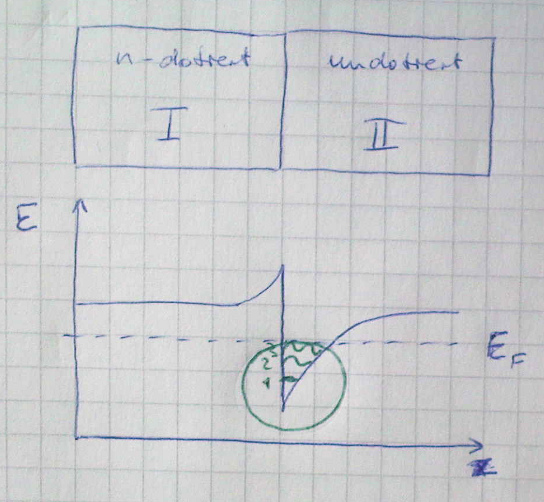
\includegraphics[width=0.75\textwidth]{kap11_01.png}

'Modulation-doped heterostructure' (engl)

z.B. 3D Metalle: \(\frac{1}{k_F}\approx 1 A\)
2DEG\(\equiv\) '2-dimensionales elektron gas'

\[\frac{1}{k_F}\approx 2\pi n)^{-\frac{1}{2}}\]

mit \(n\approx 3,5\cdot 10^{15}m^{-2}\Rightarrow \frac{1}{k}\approx 100 A\)

!Die Gitterkonstante I und II möglichst wenig unterscheiden. z.B. AlGaAs/GaAs: 

'mobility' \([\mu]\) (engl)
Beweglichkeit: \(u=\frac{|\vec v|}{\vec \epsilon} = \frac{e\tau_D}{m^*}\rightarrow \text{bis zu }10^7\frac{cm^2}{Vs}\)

z-Quantisierung: \(L_z\approx\frac{\lambda_F}{2}\approx 100 A\)

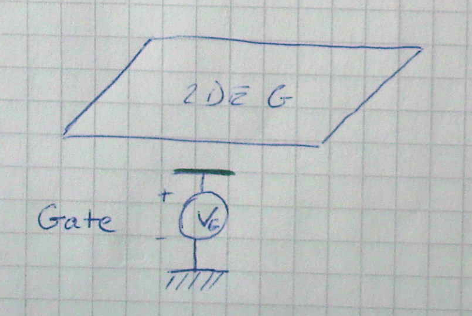
\includegraphics[width=0.75\textwidth]{kap11_02.png}

\(E_F\) turnalbe by Gate

1D system: 1D Kanal \(\rightarrow \) Quantisierung in y-Richtung


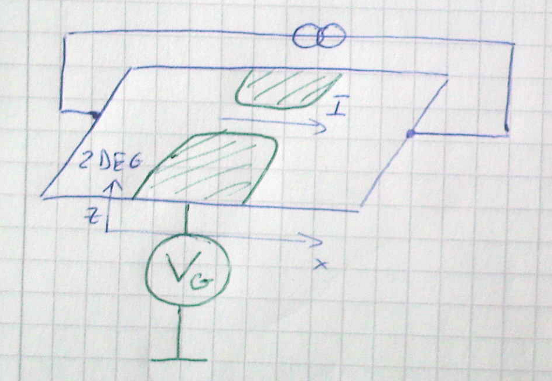
\includegraphics[width=0.75\textwidth]{kap11_03.png}

'Ballistic quantum wire' \(\rightarrow \) 1D Leiter

Im Dracht treten keine Streuprozesse auf und die Bewegung der e-nen erfolgt ballistisch (ohne Streung ohne WW).

\(\mu\)-Elektrochemisches Potential:

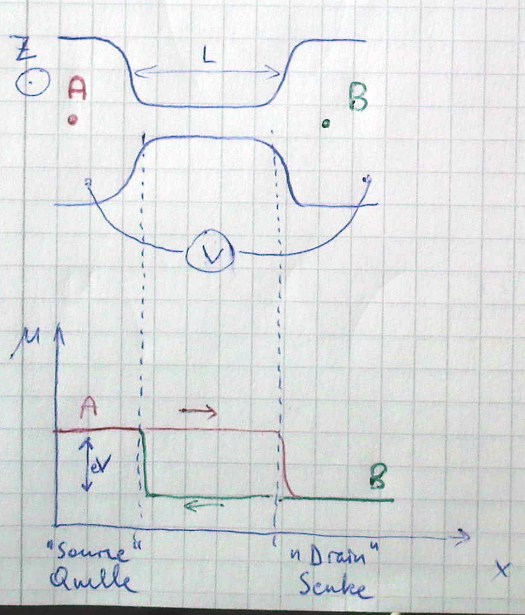
\includegraphics[width=0.75\textwidth]{kap11_04.png}

\[\Delta \mu = eV\]

Strom : 

\begin{align}
I &= ne\langle  v\rangle \\
&= \frac{1}{L}\sum_k ev_k \\
&= \frac{1}{L}\int_0^{\infty} \rho^{1D}_{k} ev_k\left[f(E+\frac{eV}{2}-f(E-\frac{eV}{2}\right]dk \\
&=\int_0^{\infty}\frac{e}{\pi}\frac{1}{\hbar}\frac{\partial E}{\partial k}dk\cdot eV \\
&=\frac{2e^2}{h}V
\end{align}

mit \(\rho^{1D}_k=\frac{2L}{2\pi}\); \(v(k)=\frac{1}{\hbar}\frac{\partial E(k)}{\partial k}\)

'conductance quantization' 

\[\left.\frac{I}{V}\right|_{\text{1 Kanal}} = \frac{2e^2}{h}\]

Leituwertsquantum; Widerstandsquantum: \(R_Q=\frac{h}{2e^2}=12,906 k\Omega\)

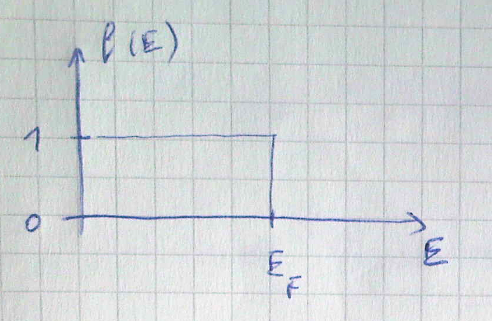
\includegraphics[width=0.75\textwidth]{kap11_05.png}


für eine Spinrichtung: \(R^\uparrow_Q =R^\downarrow_Q =25,812 k\Omega \)

\section{Niedrigdimensionale elektronensysteme: 0D; 2D}


0D: Quantumpunkte (quantum dots)


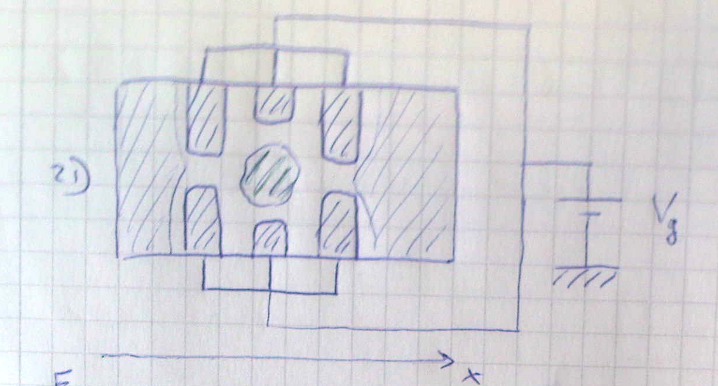
\includegraphics[width=0.75\textwidth]{kap11_06.png}

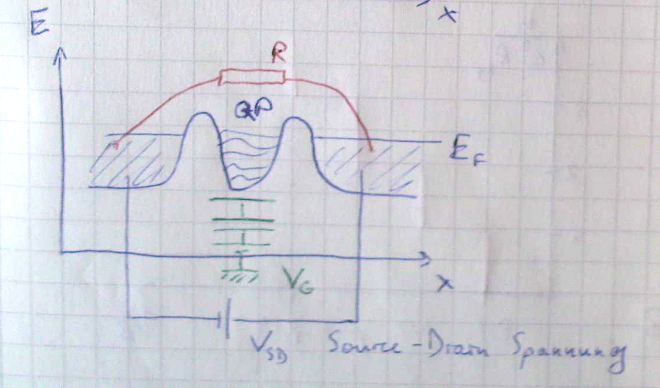
\includegraphics[width=0.75\textwidth]{kap11_07.png}

Die elektrostatische Energie: \(E(N),N\) ist die Zahl der e-nen auf dem Quantenpunkt (QP).

\[E(N) = \frac{(Ne)^2}{2C}-\phi Ne\]

mit \(\phi\propto V_g\) ist das elektrostatisches Potential
\(C\propto C_g, E(N)\) umso größer ist, je kleiner der QP und somit \(C\) ist.

Ladeenergie: \(E(N+1) = E(N)\); \((2N+1)e^2 = 2C_g eV_g\); \(V_g = \frac{e}{C_g}(N+\frac{1}{2})\)



\subsection{Coulomb-Blockade}

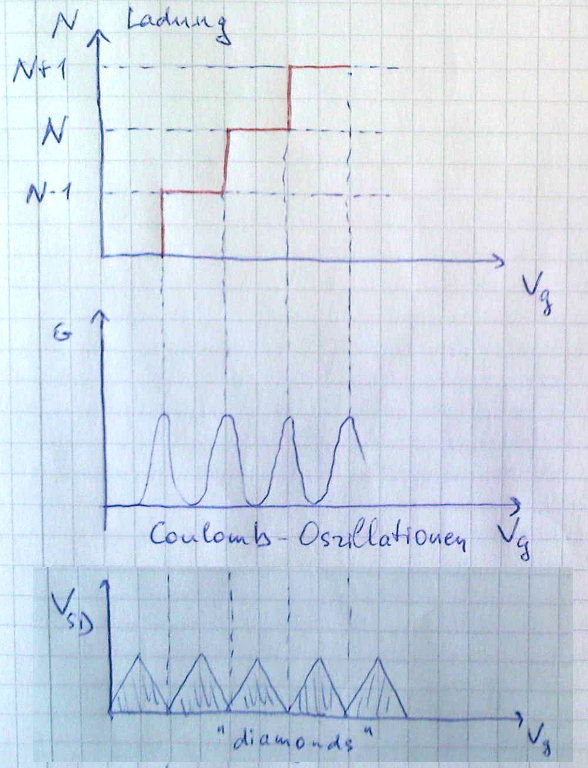
\includegraphics[width=0.75\textwidth]{kap11_08.png}

Die Energie \(\frac{e^2}{2C}=E_C\) muss bei der Gate-Spannung \(V_g = \frac{eN}{C_g}\) aufgebracht werden, wenn 1e hinzugefügt (oder entfernt) werden soll.

Wenn Source und drain sind gekoppelt mit dem Widerstand R \(\rightarrow \) Zeitskale \(\delta t \approx RC\)

\[\delta E = \frac{h}{\delta t} \simeq \frac{h}{RC} = \underbrace{\frac{e^2}{c}}_{\propto E_C}\frac{h}{e^2}\frac{1}{R} = E_C\frac{R_Q}{R}\]

\[R^\uparrow_Q = \frac{h}{e^2}=25812\Omega\]

\(\rightarrow \) Fluktationen den Coulomb-Ladeeffekt ausschmieren. Bedingungen für die Beobachtung:

\begin{itemize}
\item \(R>>R_Q\frac{h}{e^2}\)
\item \(\frac{e^2}{C}>>k_BT\)
\end{itemize}


\section{Quanten-Hall-Effekt in 2DEG}

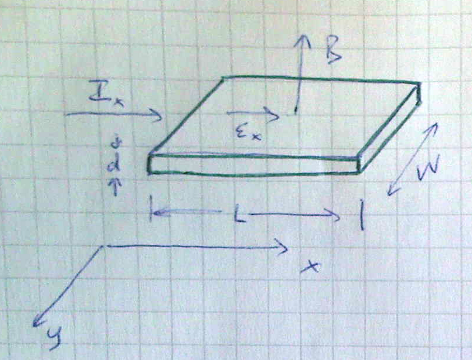
\includegraphics[width=0.75\textwidth]{kap11_09.png}

\[m \dot{\vec v} = -e(\vec{ \mathcal E} + \vec v\times\vec B)-\frac{mv}{\tau}\]

\[v_x = -\frac{e\tau}{m}(\mathcal E_x + v_yB)\]

\[v_y = -\frac{e\tau}{m}(\mathcal E_y + v_xB)\]

\[\rightarrow v_y = \begin{pmatrix}\mathcal E_x\\\mathcal E_y\end{pmatrix} =\begin{pmatrix}\rho_{xx}&\rho_{xy}\\\rho_{yx}&\rho_{yy}\end{pmatrix}\begin{pmatrix}j_x\\\j_y\end{pmatrix} \]

für isotrope Materialien \(\rho_{xx}=\rho_{yy}=\frac{m}{ne^2\tau}\); \(\rho_{xy}=\rho_{yx}=\frac{B}{ne}  \)

Mit \(j_y=0,\rightarrow \) es folgt \(\mathcal E_y = -\frac{e\tau}{m}B\mathcal E_x = -\frac{1}{ne}Bj_x = R_H Bj_x\); Hall Konstante: \(R_H = -\frac{1}{ne}\); Quanten-Hall-E. Hall-Widerstand \(R_y = |\frac{\rho_{xy}}{d}|\) \(R_x = |\frac{\rho_{xx}}{d}|\)

Entartungsgrad für jedes Landau-Niveau:

\[g_l = \frac{LW}{(2\pi)^2}(S_{l+1}-S_l)\]

mit \(S\) als Querschnittfläche von Landaurohren in der periodischen Bedingung

\[S_l = (l+\frac{1}{2})\frac{2\pi eB}{\hbar}\]

\[E_l = (l+\frac{1}{2})\hbar\omega_E+\frac{\hbar^2 k^2_{||}}{2m}\]

\[\boxed{g_l = \frac{e}{h}LWB}\]

N Elektronen verteilt auf p voll besetzen Landau Niveaus: \(N=nLWd\)

\[N= p\cdot g_l\]

\[\left.D(E)\right|_{2D}=\frac{m}{\pi \hbar^2} = const\]


\[R_y = \rho_{xy}/d = \frac{\rho_{xy}}{ned}=\frac{BLW\cancel d}{Ne\cancel d} = \frac{LWB}{pe^2LWB}=\frac{1}{p}\frac{h}{e^2}=\frac{R_Q}{p}\]

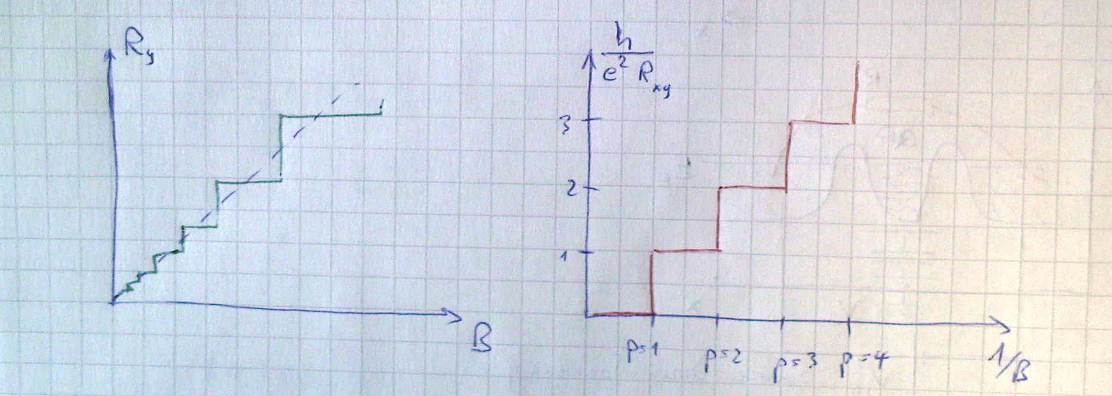
\includegraphics[width=0.75\textwidth]{kap11_10.png}


v.Klitzing entdeckt 1980, Nobel Preis 1985




